% ------------------------------------------------------------------------------
% TYPO3 CMS 7.1 - What's New (English Version)
%
% @author	Michael Schams <schams.net>
% @license	Creative Commons BY-NC-SA 3.0
% @link		http://typo3.org/download/release-notes/whats-new/
% @language	English
% ------------------------------------------------------------------------------
% LTXE-CHAPTER-UID:		e7264f0e-3f82290d-94c50cda-fb2d8e66
% LTXE-CHAPTER-NAME:	Backend User Interface
% ------------------------------------------------------------------------------

\section{BackendUI}
\begin{frame}[fragile]
	\frametitle{Interfaccia utente Backend}

	\begin{center}\huge{Capitolo 1:}\end{center}
	\begin{center}\huge{\color{typo3darkgrey}\textbf{Interfaccia utente Backend}}\end{center}

\end{frame}

% ------------------------------------------------------------------------------
% LTXE-SLIDE-START
% LTXE-SLIDE-UID:		1f5e4803-d05f9ce6-af1f194d-b18c2234
% LTXE-SLIDE-ORIGIN:	d5fddde9-b3ee31c0-f0509300-40a2928e English
% LTXE-SLIDE-TITLE:		Date/Time Picker
% LTXE-SLIDE-REFERENCE:	Breaking-62925-RemoveExtJsDateTimePicker.rst
% ------------------------------------------------------------------------------

\begin{frame}[fragile]
	\frametitle{Interfaccia utente Backend}
	\framesubtitle{Look \& Feel: componente data/orario}

	Il componente data/orario è stato sostituito con il widget basato su Bootstrap
	\begin{figure}
		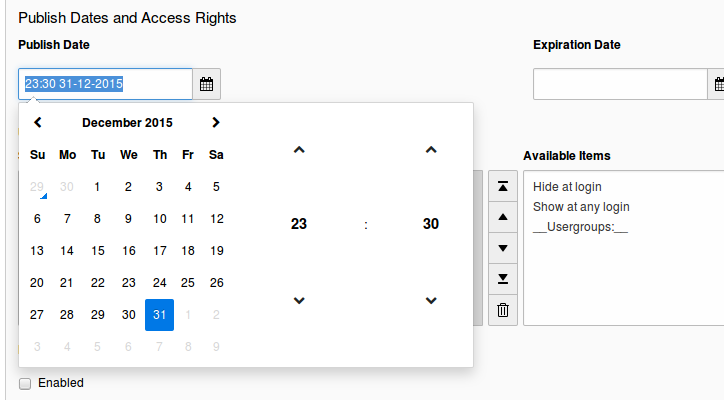
\includegraphics[width=0.75\linewidth]{BackendUserInterface/be-datepicker.png}
	\end{figure}

\end{frame}

% ------------------------------------------------------------------------------
% LTXE-SLIDE-START
% LTXE-SLIDE-UID:		3993dd98-b2a73c0c-7f727e61-bbac96d9
% LTXE-SLIDE-ORIGIN:	1c391eec-dfb1dfa6-f783ae7a-d0b214ae English
% LTXE-SLIDE-TITLE:		Functions Module
% LTXE-SLIDE-REFERENCE:	Breaking-63310-Wizard-Modules-Moved.rst
% ------------------------------------------------------------------------------

\begin{frame}[fragile]
	\frametitle{Interfaccia utente Backend}
	\framesubtitle{Look \& Feel: Modulo Funzioni}

	"Crea pagine" e "Ordina pagine" sono stati spostati in \texttt{Web => Functions}\newline
	\smaller (in TYPO3 CMS < 7.1, erano presenti in "\texttt{Web => Functions => Wizards}")

	\begin{figure}
		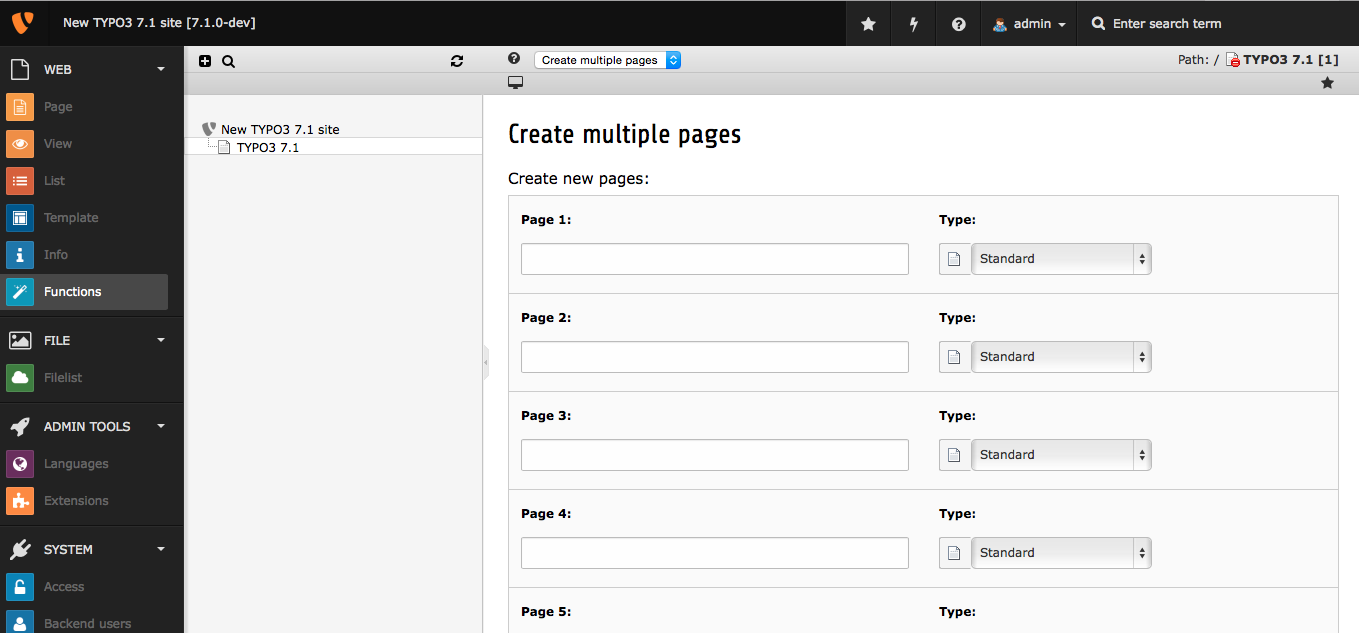
\includegraphics[width=0.80\linewidth]{BackendUserInterface/be-functions.png}
	\end{figure}


\end{frame}

% ------------------------------------------------------------------------------
% LTXE-SLIDE-START
% LTXE-SLIDE-UID:		482079d3-8543cd89-063a24a4-44469c23
% LTXE-SLIDE-ORIGIN:	dd127630-5ccc729a-835e5836-e8796962 English
% LTXE-SLIDE-TITLE:		Access Module: Leave Unchaged
% LTXE-SLIDE-REFERENCE:	Feature-15619-LeaveUnchagedInAccessModule.rst
% ------------------------------------------------------------------------------

\begin{frame}[fragile]
	\frametitle{Interfaccia utente Backend}
	\framesubtitle{Look \& Feel: Modulo Accessi}

	Il modulo \texttt{Web => Accessi} permette di lasciare invariati\newline
	i permessi utente/gruppo quando sono sovrascritti

	\begin{figure}
		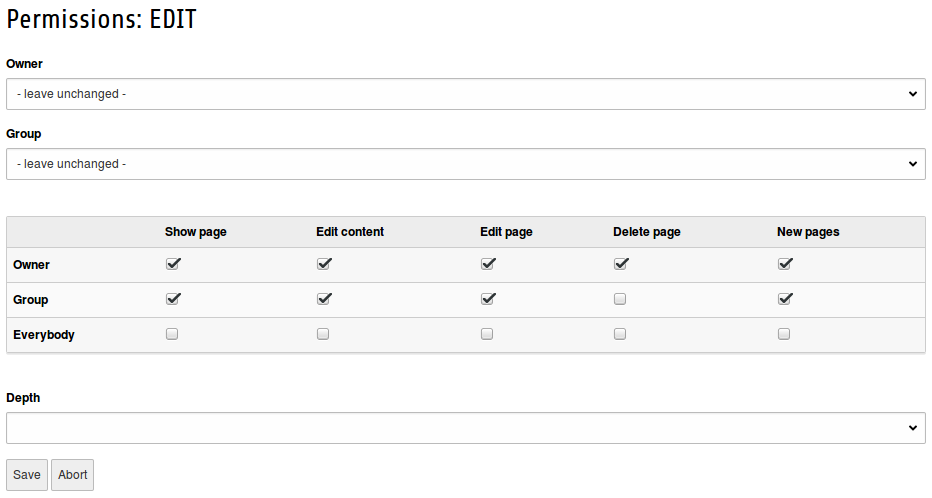
\includegraphics[width=0.75\linewidth]{BackendUserInterface/be-access.png}
	\end{figure}

\end{frame}

% ------------------------------------------------------------------------------
% LTXE-SLIDE-START
% LTXE-SLIDE-UID:		f37d7186-076d04f0-560cd2c2-4d98b594
% LTXE-SLIDE-ORIGIN:	eb6cc867-e4f5d0d3-ea06672c-7ccdf227 English
% LTXE-SLIDE-TITLE:		Icons in List Module
% LTXE-SLIDE-REFERENCE:	Feature-63207-SplitActionButtonsIntoGroups.rst
% ------------------------------------------------------------------------------

\begin{frame}[fragile]
	\frametitle{Interfaccia utente Backend}
	\framesubtitle{Look \& Feel: Icone nel modulo Lista}

	Le icone ("action buttons") nel modulo Lista sono stati divisi in due gruppi\newline
	\smaller (prima le azioni primarie (read, update, delete), seguiti dalle azioni secondarie)

	\begin{figure}
		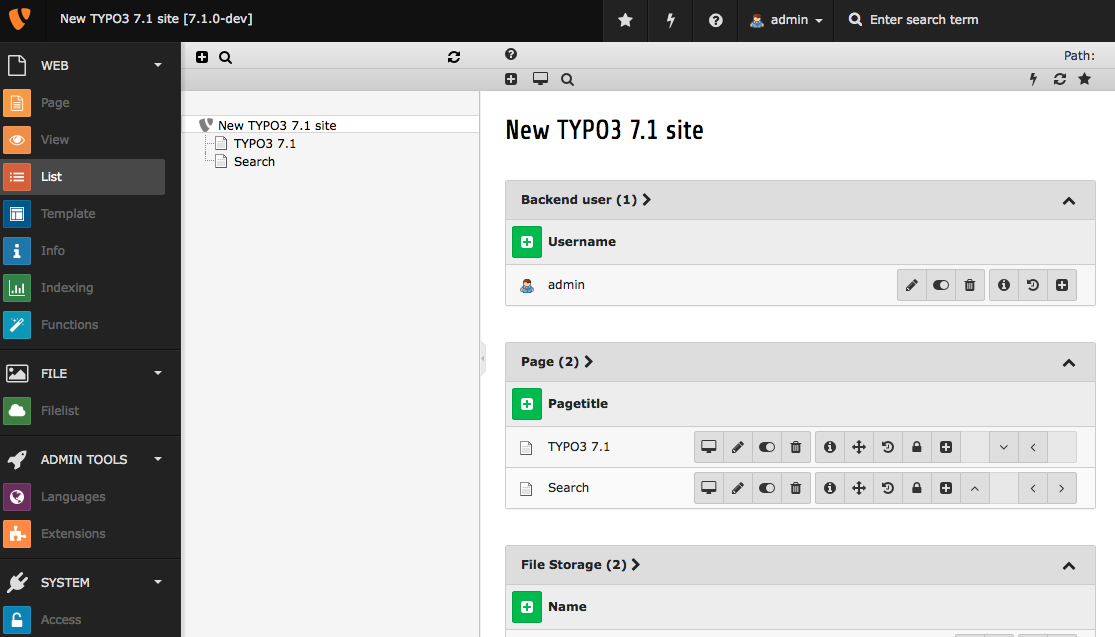
\includegraphics[width=0.75\linewidth]{BackendUserInterface/be-icons.png}
	\end{figure}

\end{frame}

% ------------------------------------------------------------------------------
